\chapter{幻方}
\label{chap:magic-square}

\epigraph{九子斜排,上下对易,左右相更,四维挺出。}{南宋·杨辉《续古摘奇算法》}

% \begin{definition}[幻方,Magic Square]
幻方(Magic Square)是一种将数字安排在正方形格子中,使每行、列和对角线上的数字和都相等的方法。若无特殊说明,这里的$n$阶幻方是指将$1,2,3,\cdots,n^2$这些数字填入到$n\times n$的格子中的幻方。
% \end{definition}

按其构造方式(参考后面示例),幻方可以分为以下三种
\begin{enumerate}
\item 奇阶幻方,即阶数为奇数的幻方;
\item 双偶阶幻方,即阶数为$4n$形式的幻方(除以2之后还是偶数);
\item 单偶阶幻方,即阶数为$4n+2$形式的幻方(除以2之后是奇数)。
\end{enumerate}

\section{幻方的性质}
\label{sec:magic-square-properties}

\begin{definition}[幻方常数]
  幻方中某一行的和称为幻方常数,也称为幻和。
\end{definition}

\begin{theorem}
  $n$阶幻方的幻和等于$\dfrac{n(1+n^2)}2$。
\end{theorem}
\begin{proof}
  设$n$阶幻方的幻和为$x$,则幻方所有数字之和为
  \begin{align*}
    1+2+3+\cdots+n^2=\frac{n^2(1+n^2)}{2}
  \end{align*}
  另一方面,每行的和为$x$,共有$n$行,从而幻方中所有数字之和也等于$xn$,从而有
  \begin{align*}
    x=\frac{n(1+n^2)}{2}&\qedhere
  \end{align*}
\end{proof}

\begin{table}[htbp]
  \centering
  \begin{tabular}{c|cccccccc}
    \toprule[2pt]
    阶数 & 3  & 4  & 5  & 6   & 7   & 8   & 9   & 10 \\\hline
         & 15 & 34 & 65 & 111 & 175 & 260 & 369 & 505\\
    \bottomrule[2pt]
  \end{tabular}
  \caption{各阶幻方常数}
  \label{tab:constant-of-some-magic-squares}
\end{table}

\section{构造方法}
\label{sec:magic-squares-construction-method}

利用南宋·杨辉《续古摘奇算法》中的写到:
\begin{quotation}
  九子斜排,上下对易,左右相更,四维挺出。
\end{quotation}
现多称为杨辉斜排法,可用于构造奇阶幻方。

\begin{example}[三阶幻方]
  将$1,2,3,4,5,6,7,8,9$几个数字填入$3\times3$的九宫格内,每个数字都要填且只能填一次,使得横竖斜三个方向的三个数字和都相同。
\end{example}
\begin{proof}[提示]
  所有填法都可由其中一种通过旋转、镜像操作可得。因此只要得出一种填法即可。其中的一个基本填法可由杨辉斜排法得出。

  首先是九子斜排。
  \newcommand\squarenode[4][blue!30]{\fill[#1](#2,#3)rectangle(#2+1,#3+1); \node at(#2+.5, #3+.5) {#4};}
  \begin{center}
    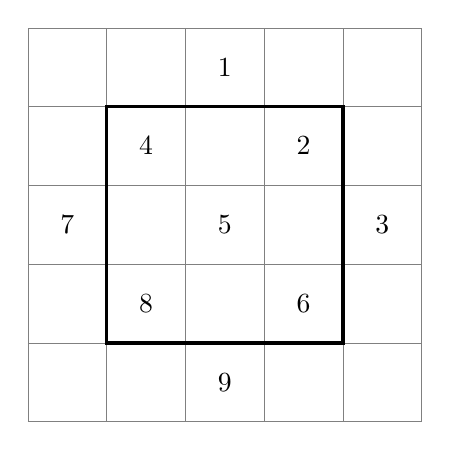
\begin{tikzpicture}[scale=1.0]
      \node at(2 + .5, 4 + .5) {$1$};
      % \squarenode[blue!30]{2}{4}{$1$};
      \node at(3 + .5, 3 + .5) {$2$};
      \node at(4 + .5, 2 + .5) {$3$};
      % \squarenode[pattern=north west lines]{4}{2}{$3$};

      \node at(1 + .5, 3 + .5) {$4$};
      \node at(2 + .5, 2 + .5) {$5$};
      \node at(3 + .5, 1 + .5) {$6$};

      \node at(0 + .5, 2 + .5) {$7$};
      % \squarenode[pattern=north west lines]{0}{2}{$7$};
      \node at(1 + .5, 1 + .5) {$8$};
      \node at(2 + .5, 0 + .5) {$9$};
      % \squarenode[blue!30]{2}{0}{$9$};

      \draw[help lines](0,0)grid(5,5);
      \draw[very thick](1,1)rectangle(4,4);
    \end{tikzpicture}
  \end{center}

  然后是上下对易,左右相更。
  \begin{center}
    \begin{tikzpicture}[scale=1.0]
      % \node at(2 + .5, 4 + .5) {$9$};
      \squarenode[fill=blue!20]{2}{4}{$9$};
      \node at(3 + .5, 3 + .5) {$2$};
      % \node at(4 + .5, 2 + .5) {$7$};
      \squarenode[pattern=north west lines,pattern color=red!50]{4}{2}{$7$};

      \node at(1 + .5, 3 + .5) {$4$};
      \node at(2 + .5, 2 + .5) {$5$};
      \node at(3 + .5, 1 + .5) {$6$};

      % \node at(0 + .5, 2 + .5) {$3$};
      \squarenode[pattern=north west lines,pattern color=red!50]{0}{2}{$3$};
      \node at(1 + .5, 1 + .5) {$8$};
      % \node at(2 + .5, 0 + .5) {$1$};
      \squarenode[fill=blue!20]{2}{0}{$1$};

      \draw[help lines](0,0)grid(5,5);
      \draw[very thick](1,1)rectangle(4,4);
    \end{tikzpicture}
  \end{center}

  最后挺出的4个方向(东南西北)压回去,或者四维挺出。
  \begin{center}
    \begin{tikzpicture}[scale=1.0]
      \begin{scope}[shift={(0,0)}]
        % \node at(2 + .5, 3 + .5) {$9$};
        \squarenode[fill=blue!20]{2}{3}{$9$};
        \draw[->](2.5,4.5)--(2.5,3.8);
        \node at(3 + .5, 3 + .5) {$2$};
        % \node at(3 + .5, 2 + .5) {$7$};
        \squarenode[pattern=north west lines,pattern color=red!50]{3}{2}{$7$};
        \draw[->](4.5,2.5)--(3.8,2.5);

        \node at(1 + .5, 3 + .5) {$4$};
        \node at(2 + .5, 2 + .5) {$5$};
        \node at(3 + .5, 1 + .5) {$6$};

        % \node at(1 + .5, 2 + .5) {$3$};
        \squarenode[pattern=north west lines,pattern color=red!50]{1}{2}{$3$};
        \draw[->](.5,2.5)--(1.2,2.5);
        \node at(1 + .5, 1 + .5) {$8$};
        % \node at(2 + .5, 1 + .5) {$1$};
        \squarenode[fill=blue!20]{2}{1}{$1$};
        \draw[->](2.5,.5)--(2.5,1.2);

        \draw[help lines](0,0)grid(5,5);
        \draw[very thick](1,1)rectangle(4,4);
      \end{scope}
      \begin{scope}[shift={(6.5,0)}]
        \draw[help lines](0,0)grid(5,5);
        \node at(2 + .5, 4 + .5) {$9$};
        \node at(4 + .5, 4 + .5) {$2$};
        \draw[->](3.75,3.75)--(4.25,4.25);
        \node at(4 + .5, 2 + .5) {$7$};

        \node at(0 + .5, 4 + .5) {$4$};
        \draw[->](1.25,3.75)--(.75,4.25);
        \node at(2 + .5, 2 + .5) {$5$};
        \node at(4 + .5, 0 + .5) {$6$};
        \draw[->](3.75,1.25)--(4.25,.75);

        \node at(0 + .5, 2 + .5) {$3$};
        \node at(0 + .5, 0 + .5) {$8$};
        \draw[->](1.25,1.25)--(.75,.75);
        \node at(2 + .5, 0 + .5) {$1$};

        \draw[very thick](1,1)rectangle(4,4);
      \end{scope}
    \end{tikzpicture}
  \end{center}
  此时幻方已成。
\end{proof}


\begin{example}[五阶幻方]\mbox{}\par
  将杨辉斜排法推广到五阶幻方。
\end{example}
\begin{proof}[提示]
首先是斜排,并取中宫。
  \begin{center}
    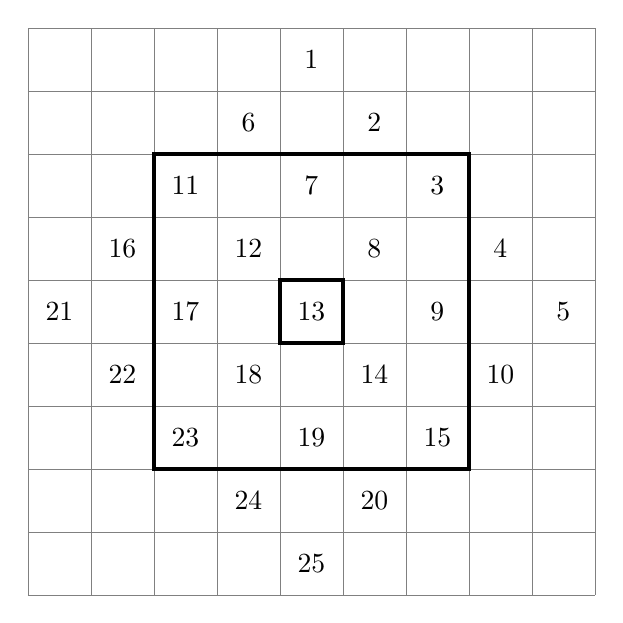
\begin{tikzpicture}[scale=.8]
      \foreach \x/\y/\v in {
        4.5/8.5/1, 5.5/7.5/2, 6.5/6.5/3, 7.5/5.5/4, 8.5/4.5/5,
        3.5/7.5/6, 4.5/6.5/7, 5.5/5.5/8, 6.5/4.5/9, 7.5/3.5/10,
        2.5/6.5/11,3.5/5.5/12,4.5/4.5/13,5.5/3.5/14,6.5/2.5/15,
        1.5/5.5/16,2.5/4.5/17,3.5/3.5/18,4.5/2.5/19,5.5/1.5/20,
        0.5/4.5/21,1.5/3.5/22,2.5/2.5/23,3.5/1.5/24,4.5/0.5/25
      }{
        \node at (\x,\y) {\v};
      }
      \draw[help lines](0,0)grid(9,9);
      \draw[very thick](4,4)rectangle(5,5);
      \draw[very thick](2,2)rectangle(7,7);
    \end{tikzpicture}
  \end{center}

  然后是上下对易。宫外上面的数字直接插入到下面,宫外下面的数字直接插入到上面。
  \begin{center}
    \begin{tikzpicture}[scale=.8]
      \foreach \x/\y in {4/8,5/7,3/7,4/3,5/2,3/2}{
        \fill[blue!20](\x,\y)rectangle(\x+1,\y+1);
      }
      \foreach \x/\y in {5/1,3/1,4/0,5/6,3/6,4/5}{
        \fill[pattern=north west lines,pattern color=red!30](\x,\y)rectangle(\x+1,\y+1);
      }
      \foreach \x/\y/\v in {
        4.5/3.5/1, 5.5/2.5/2, 6.5/6.5/3, 7.5/5.5/4, 8.5/4.5/5,
        3.5/2.5/6, 4.5/6.5/7, 5.5/5.5/8, 6.5/4.5/9, 7.5/3.5/10,
        2.5/6.5/11,3.5/5.5/12,4.5/4.5/13,5.5/3.5/14,6.5/2.5/15,
        1.5/5.5/16,2.5/4.5/17,3.5/3.5/18,4.5/2.5/19,5.5/6.5/20,
        0.5/4.5/21,1.5/3.5/22,2.5/2.5/23,3.5/6.5/24,4.5/5.5/25
      }{
        \node at (\x,\y) {\v};
      }
      \draw[help lines](0,0)grid(9,9);
      \draw[very thick](4,4)rectangle(5,5);
      \draw[very thick](2,2)rectangle(7,7);
    \end{tikzpicture}
  \end{center}

  最后是左右相更。与上下对易类似。
  \begin{center}
    \begin{tikzpicture}[scale=.8]
      \foreach \x/\y in {7/5,8/4,7/3,2/5,3/4,2/3}{
        \fill[blue!20](\x,\y)rectangle(\x+1,\y+1);
      }
      \foreach \x/\y in {1/5,0/4,1/3,6/5,5/4,6/3}{
        \fill[pattern=north west lines,pattern color=red!30](\x,\y)rectangle(\x+1,\y+1);
      }
      \foreach \x/\y/\v in {
        4.5/3.5/1, 5.5/2.5/2, 6.5/6.5/3, 2.5/5.5/4, 3.5/4.5/5,
        3.5/2.5/6, 4.5/6.5/7, 5.5/5.5/8, 6.5/4.5/9, 2.5/3.5/10,
        2.5/6.5/11,3.5/5.5/12,4.5/4.5/13,5.5/3.5/14,6.5/2.5/15,
        6.5/5.5/16,2.5/4.5/17,3.5/3.5/18,4.5/2.5/19,5.5/6.5/20,
        5.5/4.5/21,6.5/3.5/22,2.5/2.5/23,3.5/6.5/24,4.5/5.5/25
      }{
        \node at (\x,\y) {\v};
      }
      \draw[help lines](0,0)grid(9,9);
      \draw[very thick](4,4)rectangle(5,5);
      \draw[very thick](2,2)rectangle(7,7);
    \end{tikzpicture}
  \end{center}

  幻方已成,无需四维挺出。
\end{proof}

\begin{question}[花16图]
  作出一个四阶($4\times 4$)幻方。
\end{question}
\begin{proof}[提示]杨辉斜排法只适用于奇数阶幻方。下面方法只适用于$4n$阶幻方。首先顺序排列16个数字,然后保持两对角线上数字不动,其余数字与关于中心点对称的数字对调,幻方即成。
  \begin{center}
    \begin{tikzpicture}[scale=.8]
      \begin{scope}[shift={(0,0)}]
        \foreach \x/\y in {0/0,1/1,2/2,3/3}{
          \fill[blue!20](\x,\y)rectangle(\x+1,\y+1);
        }
        \foreach \x/\y in {0/3,1/2,2/1,3/0}{
          \fill[red!20](\x,\y)rectangle(\x+1,\y+1);
        }
        \foreach \x/\y/\v in {
          0/3/1, 1/3/2, 2/3/3, 3/3/4,
          0/2/5, 1/2/6, 2/2/7, 3/2/8,
          0/1/9, 1/1/10,2/1/11,3/1/12,
          0/0/13,1/0/14,2/0/15,3/0/16
        }{
          \node at (\x+.5,\y+.5) {\v};
        }
        \draw[help lines](0,0)grid(4,4);
        \node at(2,-1) {对角线上的不动};
      \end{scope}
      \node at (5,2){\huge$\implies$};
      \begin{scope}[shift={(6,0)}]
        \foreach \x/\y in {1/3,2/0}{
          \fill[blue!20](\x,\y)rectangle(\x+1,\y+1);
        }
        \foreach \x/\y in {2/3,1/0}{
          \fill[pattern=north west lines,pattern color=red!30](\x,\y)rectangle(\x+1,\y+1);
        }
        \draw[help lines,<->](1.5,3)--(2.5,1);
        \draw[help lines,<->](2.5,3)--(1.5,1);
        \foreach \x/\y/\v in {
          0/3/1, 1/3/15,2/3/14,3/3/4,
          0/2/5, 1/2/6, 2/2/7, 3/2/8,
          0/1/9, 1/1/10,2/1/11,3/1/12,
          0/0/13,1/0/3, 2/0/2, 3/0/16
        }{
          \node at (\x+.5,\y+.5) {\v};
        }
        \draw[help lines](0,0)grid(4,4);
        \fill(2,2)circle(2pt);
        \node at(2,-1) {对调};
      \end{scope}
      \node at (11,2){\huge$\implies$};
      \begin{scope}[shift={(12,0)}]
        \foreach \x/\y in {0/2,3/1}{
          \fill[blue!20](\x,\y)rectangle(\x+1,\y+1);
        }
        \foreach \x/\y in {0/1,3/2}{
          \fill[pattern=north west lines,pattern color=red!30](\x,\y)rectangle(\x+1,\y+1);
        }
        \draw[help lines,<->](1,2.5)--(3,1.5);
        \draw[help lines,<->](1,1.5)--(3,2.5);
        \foreach \x/\y/\v in {
          0/3/1, 1/3/15,2/3/14,3/3/4,
          0/2/12,1/2/6, 2/2/7, 3/2/9,
          0/1/8, 1/1/10,2/1/11,3/1/5,
          0/0/13,1/0/3, 2/0/2, 3/0/16
        }{
          \node at (\x+.5,\y+.5) {\v};
        }
        \draw[help lines](0,0)grid(4,4);
        \fill(2,2)circle(2pt);
        \node at(2,-1) {对调};
      \end{scope}
    \end{tikzpicture}
  \end{center}
  此方法只适用于$4n$阶幻方。
\end{proof}

\begin{example}[$4n$阶幻方]
  与$4$阶幻方类似,首先划分为$4\times4$的小方块,每个小方块中的对角线元素不动;然后整体考虑,其余元素作关于幻方中心点的对调。下面第$2$个图中只对调了其中的$12$个元素,其余的请自行补充完整。
  \begin{center}
    \begin{tikzpicture}[scale=.7]
      \begin{scope}[shift={(0,0)}]
        \foreach \x/\y/\color in {0/0/blue!20, 4/0/yellow!40, 0/-4/red!20, 4/-4/green!20}{
        \begin{scope}[shift={(\x,\y)}]
          \foreach \x in {0,1,2,3}{
            \fill[color=\color](\x,-\x)rectangle(\x+1,-\x-1);
            \fill[pattern=crosshatch,pattern color=\color](\x,\x-4)rectangle(\x+1,\x-3);
          }
        \end{scope}
        }

        \foreach \x in {0,1,2,3,4,5,6,7}{
          \foreach \y in {0,1,2,3,4,5,6,7}{
            \pgfmathtruncatemacro{\v}{1+\x+8*\y}%
            \node at (\x+.5, -\y-.5) {\v};
          }
        }

        \draw[help lines](0,0)grid(8,-8);
        \draw[very thick](0,0)rectangle(8,-8);
        \draw[very thick](4,0)--(4,-8) (0,-4)--(8,-4);
      \end{scope}

      \begin{scope}[shift={(9.5,0)}]
        % \foreach \x/\y/\color in {0/0/blue!20, 4/0/yellow!40, 0/-4/red!20, 4/-4/green!20}{
        % \begin{scope}[shift={(\x,\y)}]
        %   \foreach \x in {0,1,2,3}{
        %     \fill[color=\color](\x,-\x)rectangle(\x+1,-\x-1);
        %     \fill[pattern=crosshatch,pattern color=\color](\x,\x-4)rectangle(\x+1,\x-3);
        %   }
        % \end{scope}
        % }
        \foreach \x/\y/\color in {1/0,6/-7}{
          \fill[color=blue!20](\x,\y)rectangle(\x+1,\y-1);
        }
        \draw[help lines,<->](1.5,-1)--(6.5,-7);

        \foreach \x/\y/\color in {2/0,5/-7}{
          \fill[pattern=north west lines,pattern color=red!20](\x,\y)rectangle(\x+1,\y-1);
        }
        \draw[help lines, <->](2.5,-1)--(5.5,-7);

        \foreach \x/\y/\color in {5/0,2/-7}{
          \fill[color=red!20](\x,\y)rectangle(\x+1,\y-1);
        }
        \draw[help lines,<->](5.5,-1)--(2.5,-7);

        \foreach \x/\y/\color in {6/0,1/-7}{
          \fill[pattern=north west lines,pattern color=green!30](\x,\y)rectangle(\x+1,\y-1);
        }
        \draw[help lines, <->](6.5,-1)--(1.5,-7);

        \foreach \x in {0,1,2,3,4,5,6,7}{
          \foreach \y in {0,1,2,3,4,5,6,7}{
            \pgfmathtruncatemacro{\v}{1+\x+8*\y}%
            \ifnum2=\v\node at (\x+.5, -\y-.5) {63};
            \else \ifnum\v=3 \node at (\x+.5, -\y-.5) {62};
            \else \ifnum\v=62\node at (\x+.5, -\y-.5) {3};
            \else \ifnum\v=63\node at (\x+.5, -\y-.5) {2};
            \else \ifnum\v=6 \node at (\x+.5, -\y-.5) {59};
            \else \ifnum\v=7 \node at (\x+.5, -\y-.5) {58};
            \else \ifnum\v=58\node at (\x+.5, -\y-.5) {7};            
            \else \ifnum\v=59\node at (\x+.5, -\y-.5) {6};

            \else \ifnum\v=30\node[scale=.8,fill=blue!20] at (\x+.5, -\y-.5) {35};
            \else \ifnum\v=35\node[scale=.8,fill=blue!20] at (\x+.5, -\y-.5) {30};
            \else \ifnum\v=27\node[scale=.6,circle,draw=black] at (\x+.5, -\y-.5) {38};
            \else \ifnum\v=38\node[scale=.6,circle,draw=black] at (\x+.5, -\y-.5) {27};
            \else\node at (\x+.5, -\y-.5) {\v};
            \fi\fi\fi\fi\fi\fi\fi\fi\fi\fi\fi\fi
          }
        }

        \draw[help lines](0,0)grid(8,-8);
        \draw[very thick](0,0)rectangle(8,-8);
        \draw[very thick](4,0)--(4,-8) (0,-4)--(8,-4);
      \end{scope}
    \end{tikzpicture}
  \end{center}

\end{example}


\begin{example}[$4n+2$阶幻方]
  作出一个六阶幻方。
\end{example}
\begin{proof}[提示]
  用加边法。先用中间的数字做成一个$4n$的幻方,需要$4n\times 4n=16n^2$个元素。$4n+2$阶幻方共有$(4n+2)\times(4n+2)=16n^2+16n+4$个元素,比$4n$阶幻方多出$16n+4$个元素,前后各空$8n+2$个。
  \begin{align*}
    \underbrace{1,2,\cdots,K}_{K\text{个元素}},\underbrace{K+1,K+2,\cdots,16n^2+K}_{16n^2\text{个元素}},
    \underbrace{16n^2+K+1,\cdots,(4n+2)^2}_{K\text{个元素}}
  \end{align*}
  其中$K\equiv 8n+2$,对于六阶幻方,$n=1$,$K=8n+2=10$。先用$1,2,\cdots,16n^2$做出$4n$阶幻方,再对其中每个数字加上$K$,得到$4n+2$阶幻方的内部,再将剩余的数字在外面填一圈。
  \begin{center}
    \begin{tikzpicture}[scale=1.0]
      \begin{scope}[shift={(0,0)}]
        \foreach \x/\y/\v in {
          1/4/1, 2/4/15,3/4/14,4/4/4,
          1/3/12,2/3/6, 3/3/7, 4/3/9,
          1/2/8, 2/2/10,3/2/11,4/2/5,
          1/1/13,2/1/3, 3/1/2, 4/1/16
        }{
          \node at (\x+.5,\y+.5) {\v};
        }
        \draw[help lines](1,1)grid(5,5);
        % \draw[very thick](1,1)rectangle(5,5);
        \fill(3,3)circle(2pt);
        \node at(3,.5){$4$阶幻方};
      \end{scope}
      \node at(6.5,3){$\xrightarrow[\text{加边框}]{\text{每个元素加10}}$};
      \begin{scope}[shift={(8,0)}]
        \foreach \x/\y/\v in {
          1/4/11,2/4/25,3/4/24,4/4/14,
          1/3/22,2/3/16,3/3/17,4/3/19,
          1/2/18,2/2/20,3/2/21,4/2/15,
          1/1/23,2/1/13,3/1/12,4/1/26
        }{
          \node at (\x+.5,\y+.5) {\v};
        }
        \draw[help lines](0,0)grid(6,6);
        \draw[very thick](1,1)rectangle(5,5);
        \fill(3,3)circle(2pt);        
      \end{scope}
    \end{tikzpicture}
  \end{center}
  将$1,2,3,\cdots,10$及$27,28,29,\cdots,36$这20个数字在外面填一圈,可得到六阶幻方。六阶幻方的幻和是$111$,四阶幻方的幻和是$34$,从而按上述方法得到的六阶幻方的内核幻方的和为$34+10\times4=74$,从而上下、左右以及对角点的和必须是$111-74=37$,从而剩余的数字可分为以下10组组合:
  \begin{align*}\renewcommand*{\arraystretch}{.9}
  \begin{array}{cccccccccc}
    1  & 2  & 3  & 4  & 5  & 6  & 7  & 8  & 9  & 10\\
    \Updownarrow & \Updownarrow & \Updownarrow & \Updownarrow & \Updownarrow & \Updownarrow & \Updownarrow & \Updownarrow & \Updownarrow & \Updownarrow\\
    36 & 35 & 34 & 33 & 32 & 31 & 30 & 29 & 28 & 27
  \end{array}
  \end{align*}
  显然边框上每行每列都必须包含3个小数与3个大数,否则该行或该列的和不会为$111$。先确定四个角,把最大与最小的4个数字按分组填入,使对角线的和等于幻和。
  \begin{center}
    \begin{tikzpicture}[scale=1.0]
      \begin{scope}[shift={(0,0)}]
        \foreach \x/\y/\v in {
          1/4/1, 2/4/15,3/4/14,4/4/4,
          1/3/12,2/3/6, 3/3/7, 4/3/9,
          1/2/8, 2/2/10,3/2/11,4/2/5,
          1/1/13,2/1/3, 3/1/2, 4/1/16
        }{
          \node at (\x+.5,\y+.5) {\v};
        }
        \draw[help lines](1,1)grid(5,5);
        % \draw[very thick](1,1)rectangle(5,5);
        \fill(3,3)circle(2pt);
        \node at(3,.5){$4$阶幻方};
      \end{scope}
      \node at(6.5,3){$\xrightarrow[\text{加边框}]{\text{每个元素加10}}$};
      \begin{scope}[shift={(8,0)}]
        \foreach \x/\y/\v in{0/5/1,5/0/36}{
          \fill[color=blue!20](\x+.5,\y+.5)circle(.5);
          \node at(\x+.5,\y+.5){\v};
        }
        \foreach \x/\y/\v in{5/5/2,0/0/35}{
          \fill[pattern=north west lines,pattern color=red!20](\x,\y)rectangle(\x+1,\y+1);
          \node at(\x+.5,\y+.5){\v};
        }
        \foreach \x/\y/\v in {
          1/4/11,2/4/25,3/4/24,4/4/14,
          1/3/22,2/3/16,3/3/17,4/3/19,
          1/2/18,2/2/20,3/2/21,4/2/15,
          1/1/23,2/1/13,3/1/12,4/1/26
        }{
          \node at (\x+.5,\y+.5) {\v};
        }
        \draw[help lines](0,0)grid(6,6);
        \draw[very thick](1,1)rectangle(5,5);
        \fill(3,3)circle(2pt);        
      \end{scope}
    \end{tikzpicture}
  \end{center}  

  考虑最上面的边框,$1,2$最小,要使其和达到平均数,将剩余最大的两个数字$34,33$填入,分组中与$34,33$对应的$3,4$则相应的填入到最下面一行。
  \begin{center}
    \begin{tikzpicture}[scale=1.0]
      \begin{scope}[shift={(0,0)}]
        \foreach \x/\y/\v in{0/5/1,5/0/36,0/0/35,5/5/2}{
          \node at(\x+.5,\y+.5){\v};
        }
        \foreach \x/\y/\v in{2/0/4,2/5/33}{
          \fill[pattern=north west lines,pattern color=red!20](\x,\y)rectangle(\x+1,\y+1);
          \node at(\x+.5,\y+.5){\v};
        }
        \foreach \x/\y/\v in{1/0/3,1/5/34}{
          \fill[color=blue!20](\x+.5,\y+.5)circle(.5);
          \node at(\x+.5,\y+.5){\v};
        }
        \foreach \x/\y/\v in {
          1/4/11,2/4/25,3/4/24,4/4/14,
          1/3/22,2/3/16,3/3/17,4/3/19,
          1/2/18,2/2/20,3/2/21,4/2/15,
          1/1/23,2/1/13,3/1/12,4/1/26
        }{
          \node at (\x+.5,\y+.5) {\v};
        }
        \draw[help lines](0,0)grid(6,6);
        \draw[very thick](1,1)rectangle(5,5);
        \fill(3,3)circle(2pt);        
      \end{scope}
    \end{tikzpicture}
  \end{center}
  此时最上面一行剩余2个空格,还需填入一个大数和一个小数,可选项为$9,32$或者$10,31$。随便选一组,此处选$10,31$(若有兴趣,请自行完成$9,32$的情况),同时在最下行填入与之对应的数字。此时剩余的数字为
  \begin{align*}\renewcommand*{\arraystretch}{.9}
  \begin{array}{cccccccccc}
    \tikzmark{tsa}{1}  & \tikzmark{tsb}{2}  & \tikzmark{tsc}{3}  & \tikzmark{tsd}{4}  & 5  & \tikzmark{tse}{6}  & 7  & 8  & 9  & \tikzmark{tsf}{10}\\
    \Updownarrow & \Updownarrow & \Updownarrow & \Updownarrow & \Updownarrow & \Updownarrow & \Updownarrow & \Updownarrow & \Updownarrow & \Updownarrow\\
    \tikzmark{tea}{36} & \tikzmark{teb}{35} & \tikzmark{tec}{34} & \tikzmark{ted}{33} & 32 & \tikzmark{tee}{31} & 30 & 29 & 28 & \tikzmark{tef}{27}
  \end{array}
  \end{align*}
  \foreach \s/\e in{tsa/tea,tsb/teb,tsc/tec,tsd/ted,tse/tee,tsf/tef}{
    \DrawVLine[black,opacity=.5]{\s}{\e}
  }

  \begin{center}
    \begin{tikzpicture}[scale=1.0]
      \begin{scope}[shift={(0,0)}]
        \foreach \x/\y/\v in{0/5/1,5/0/36,0/0/35,5/5/2,1/5/34,2/5/33,2/0/4,1/0/3}{
          \node at(\x+.5,\y+.5){\v};
        }
        \foreach \x/\y/\v in{3/5/10,3/0/27}{
          \fill[pattern=north west lines,pattern color=red!20](\x,\y)rectangle(\x+1,\y+1);
          \node at(\x+.5,\y+.5){\v};
        }
        \foreach \x/\y/\v in{4/5/31,4/0/6}{
          \fill[color=blue!20](\x+.5,\y+.5)circle(.5);
          \node at(\x+.5,\y+.5){\v};
        }
        \foreach \x/\y/\v in {
          1/4/11,2/4/25,3/4/24,4/4/14,
          1/3/22,2/3/16,3/3/17,4/3/19,
          1/2/18,2/2/20,3/2/21,4/2/15,
          1/1/23,2/1/13,3/1/12,4/1/26
        }{
          \node at (\x+.5,\y+.5) {\v};
        }
        \draw[help lines](0,0)grid(6,6);
        \draw[very thick](1,1)rectangle(5,5);
        \fill(3,3)circle(2pt);        
      \end{scope}

      \begin{scope}[shift={(7,0)}]
        \foreach \x/\y/\v in{0/5/1,5/0/36,0/0/35,5/5/2,1/5/34,2/5/33,2/0/4,1/0/3,3/5/10,3/0/27,4/5/31,4/0/6}{
          \node at(\x+.5,\y+.5){\v};
        }
        \foreach \x/\y/\v in{0/4/7,5/4/30}{
          \fill[pattern=north west lines,pattern color=red!20](\x,\y)rectangle(\x+1,\y+1);
          \node at(\x+.5,\y+.5){\v};
        }
        \foreach \x/\y/\v in{0/3/8,5/3/29}{
          \fill[color=blue!20](\x+.5,\y+.5)circle(.5);
          \node at(\x+.5,\y+.5){\v};
        }

        % \foreach \x/\y/\v in{0/2/32,5/2/5}{
        %   \fill[pattern=north east lines,pattern color=blue!20](\x+.5,\y)--(\x+1,\y+.5)--(\x+.5,\y+1)--(\x,\y+.5)--cycle;
        %   \node at(\x+.5,\y+.5){\v};
        % }
        % \foreach \x/\y/\v in{0/1/28,5/1/9}{
        %   \fill[color=red!20](\x+.25,\y+.25)rectangle(\x+.75,\y+.75);
        %   \node at(\x+.5,\y+.5){\v};
        % }

        \foreach \x/\y/\v in {
          1/4/11,2/4/25,3/4/24,4/4/14,
          1/3/22,2/3/16,3/3/17,4/3/19,
          1/2/18,2/2/20,3/2/21,4/2/15,
          1/1/23,2/1/13,3/1/12,4/1/26
        }{
          \node at (\x+.5,\y+.5) {\v};
        }
        \draw[help lines](0,0)grid(6,6);
        \draw[very thick](1,1)rectangle(5,5);
        \fill(3,3)circle(2pt);        
      \end{scope}
    \end{tikzpicture}
  \end{center}

  此时最左列与最右列都剩余4个空格,都需要填入两个小数和两个大数。其排列组合只有若干几种,排除后可得最终结果。(若不用排除法是否有更简单的方法?)
\end{proof}

\section{练一练}
\label{sec:yanghui-method-exercise}

\begin{question}[七阶幻方]
  将杨辉斜排法推广到七阶($7\times 7$)幻方。
\end{question}

\begin{question}
  作出一种$8$阶幻方。
\end{question}